\chapter{System Design}

The system model is developed in three stages. %
The first two stages were developed in MATLAB, %
and consist of a time invariant model %
for simulating the convergence behaviour of %
the LMS algorithms, and a time varying %
model for showing the tracking performance %
in the environment proposed in section %
\ref{sec:MotivatingScenario}. The %
final stage was developed in LabView on the %
National Instruments Universial Software Radio %
Platform (USRP) model 2943R and presents %
a hardware proof of concept for adaptive %
filtering in slowly time varying channels. %
This section will be dedicated to developing %
the system models. Chapter \ref{chap:Results} %
will develop the results that I collected %
and compare them with whats available in the %
literature.

\section{Time Invariant System Model}
\FloatBarrier
\begin{figure}[ht]
	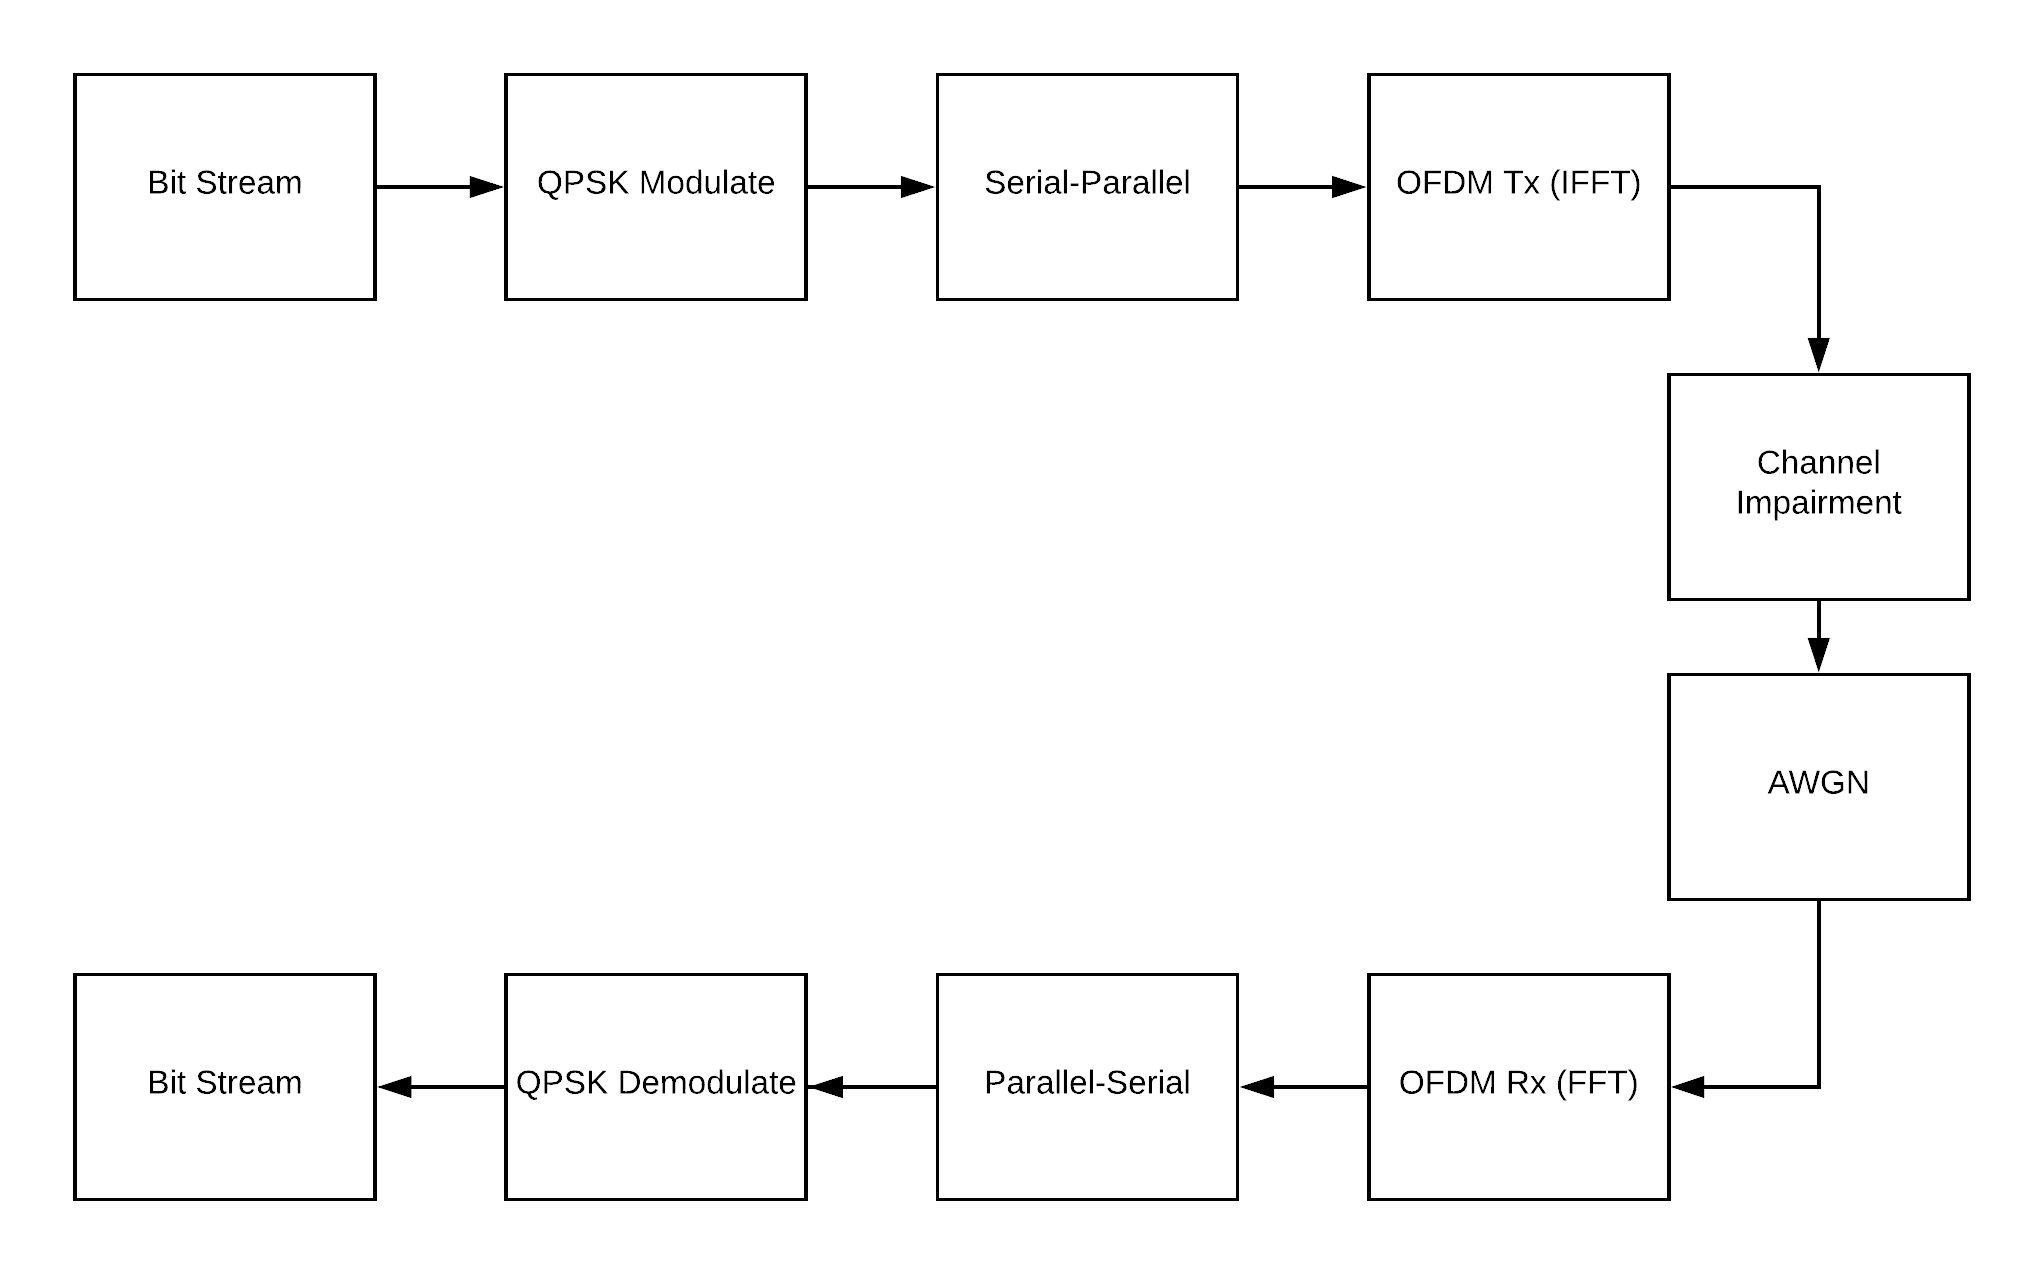
\includegraphics[width=\textwidth]{./%
	Figures/System/SystemModel.png}
	\caption{System Model}
	\label{fig:SysModel}
\end{figure}
Figure \ref{fig:SysModel} depicts the general %
outline of the system model that has been %
developed. This section will focus on %
developing all the components that will %
be common to all the later sections as %
well as section specific components.
\FloatBarrier
The primary aim of the time invariant %
model was to establish the convergence %
of the LMS algorithm with an OFDM %
transmission scheme, equalising in the %
\emph{frequency} domain.
\begin{figure}[ht]
	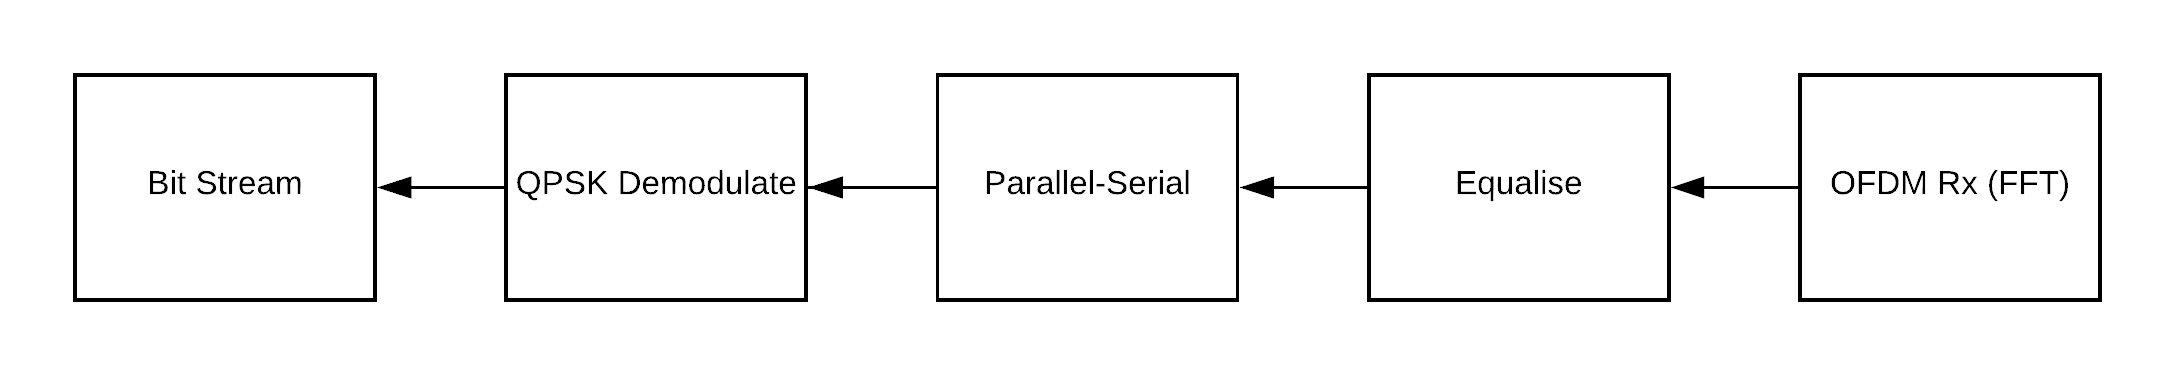
\includegraphics[width=\textwidth]{./%
	Figures/System/RxEqualisation.png}
	\caption{Added equalisation step}
	\label{fig:RxEqualiser}
\end{figure}
Figure \ref{fig:RxEqualiser} illustrates %
the location of the equaliser in this model, %
immediately after the FFT and before the %
parallel to serial step. By designing %
the OFDM subcarrier bandwidth to be %
significantly less than the coherence %
bandwidth of the fading channel a simple %
version of the LMS filter with only one %
filter coefficient can be assigned to %
each subcarrier for equalisation as %
illustrated in figure \ref{fig:Frequency%
LMS}
\FloatBarrier
\begin{figure}[ht]
	\centering
	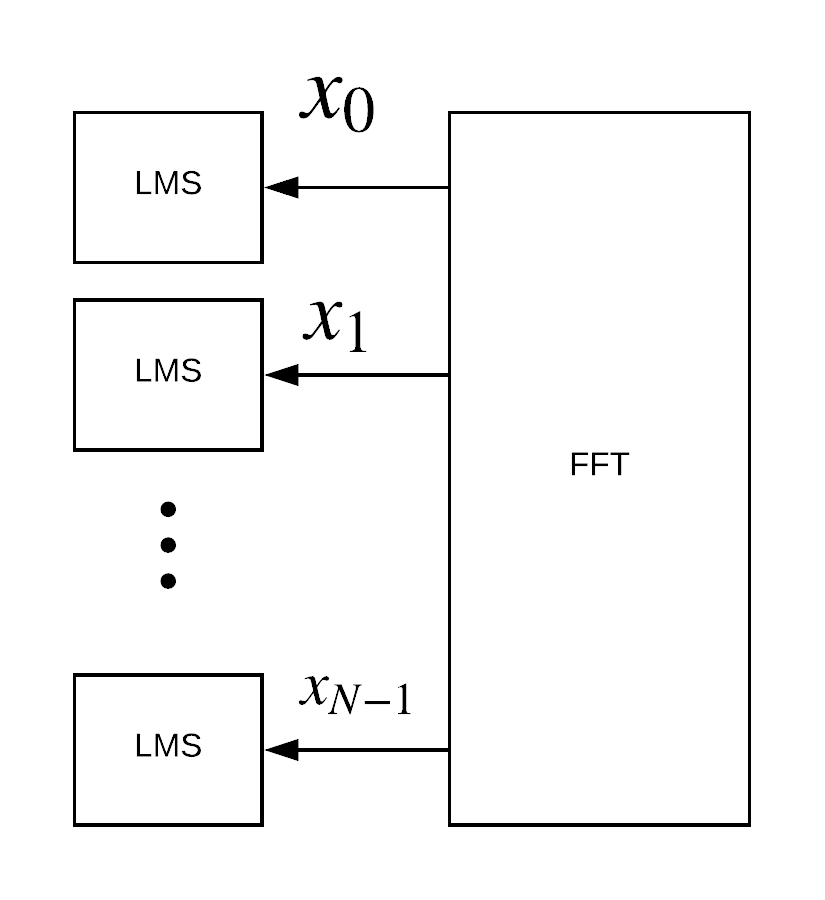
\includegraphics[width=0.5\textwidth]{./%
	Figures/System/FrequencyDomainLMS.png}
	\caption{Single Tap LMS on each Sub%
	carrier}
	\label{fig:FrequencyLMS}
\end{figure}
\FloatBarrier
\subsection{Bit Stream}
The bit stream needs to be selected to model %
a believable source of data. It can be shown %
that without further information, data %
in digital communications systems can be %
modeled as a Bernoulli distribution. %TODO: Cite this
My model simulates this using MATLAB's in-built %
\texttt{randi} function which generates %
a random vector $\bold{X}$ where each %
random variable $X$ can take on values from %
a user defined set of integers and is %
uniformly distributed, i.e. where each integer %
has an equally likely chance of occuring. In %
the special case of the Bernoulli distribution %
the set of integers can be defined as $\{0,1\}$.

\subsection{QPSK Modulation and Demodulation}
\FloatBarrier
QPSK or Quadrature Phase Shift Keying is a popular %
modulation scheme. I've chosen to use it primarily %
for its simplicity but also because it contains both
an in-phase and a quadrature component, which are%
the elements required to construct %
Quadrature Amplitude Modulation (QAM) %
which is the current modulation scheme employed %
in 4G systems % TODO: Find a citation for this.
and is likely to be used in 5G schemes.

\begin{figure}[ht]
	\centering
	\includegraphics[width=0.7\textwidth]{./%
	Figures/System/QPSKScatterplotWithA%
	WGN.png}
	\caption{QPSK Constellation, red stars %
	indicate constellation points, blue %
	points are due to noise}
	\label{fig:QPSKConstellation}
\end{figure}

Figure \ref{fig:QPSKConstellation} shows what %
a QPSK constellation looks like and how a %
received signal might appear when AWGN has %
been added to it. To normalise that average %
symbol energy to 1 the constellation points %
are defined at $\{\frac{\sqrt{2}}{2} + \frac{%
\sqrt{2}}{2}i, \frac{\sqrt{2}}{2} - %
\frac{\sqrt{2}}{2}i, -\frac{\sqrt{2}%
}{2} + \frac{\sqrt{2}}{2}i, %
-\frac{\sqrt{2}}{2} - \frac{\sqrt{2}%
}{2}i\}$ such that when the average %
energy is evaluated
\begin{align}
	E\left[E_s\right] = \frac{1}{4} \sum_{k=1}^{4} %
	\lvert E_{s_{k}} \rvert = 1
\end{align}
where $E_{s_{k}}$ is the symbol energy of the the %
$k\text{th}$ element in the symbol set. A QPSK %
modulation scheme has a symbol set of size $4$. %
So is capable of transmitting $log_{2}(4)$ bits %
per symbol. In general a M-QAM modulation scheme %
is able to transmit $log_{2}(M)$ bits per symbol. %
A grey mapping between pairs of bits to the QPSK %
constellation needs to be chosen so that symbol %
errors that are due to the received symbol mapping %
incorrectly to a neighbouring symbol than what was %
desired will introduce only one bit error instead %
of multiple, it can be shown that grey mapping %
minimises the bit error rate caused by %
symbol errors. %TODO: Find a citation for grey mapping

MATLAB's Communications System Toolbox offers %
a system object name \texttt{QPSKModulator} which %
will perform the grey mapping of pairs of bits in a %
bit stream to QPSK constellation points and perform %
the energy normalisation.

%TODO: Finish up QPSK Demodulation

\subsection{OFDM}

%TODO: Finish describing MATLAB's OFDM
% system object since it's reasonably 
% complicated

\subsection{AWGN}

\subsection{Channel Impairment}

\subsection{Equalisation}


\section{Time Varying System Model}

%TODO: Insert my MATLAB code here for generating 
% a random frame.


%NOTE: Rigourously justify every use of a MATLAB library function.

\section{USRP Implementation of the Time Varying System Model}

%TODO: Carefully develop the USRP implementation

